\section{Primjeri}
U ovom poglavlju demonstriramo rad aplikacije na pokaznoj bazi,
dajemo primjere tipičnih upita i prikazujemo njihove rezultate.

\subsection{Pokazna baza} \label{subsec:pokazna}
Za potrebe demonstracije, stvaramo bazu s nekoliko
paketa:
\begin{itemize}
\item ovaj projekt (v.~\cite{repo}),
\item humanize (URL: \url{https://github.com/jmoiron/humanize}),
\item Requests (URL: \url{https://github.com/psf/requests}),
\item Seaborn (URL: \url{https://github.com/seaborn/seaborn}) i
\item PyMC (URL: \url{https://github.com/pymc-devs/pymc}).
\end{itemize}

\subsection{Primjeri upita} \label{subsec:primjer}
Razmotrimo nekoliko zanimljivih upita:
\begin{enumerate}

\item Nađimo broj vrhova po tipu unutar svakog od paketa. Rezultat je prikazan
u tablici~\ref{tab:upit1}. Ostvarujemo ga sljedećim upitom:
\begin{lstlisting}
MATCH (p: Package)
WHERE NOT EXISTS ((p)-[:WITHIN_SCOPE]->())
MATCH (p)<-[:(WITHIN_SCOPE | ATTRIBUTE)*0..]-(n)
RETURN p.fullname AS ime_paketa, labels(n)[0] AS tip, COUNT(*) AS broj;
\end{lstlisting}
Rezultati svih upita mogu se naći, kao CSV ili PNG, unutar \texttt{tex/assets}
folderu unutar repozitorija projekta.

\item Nađimo hijerarhiju paketa i modula unutar Seaborn-a. Rezultat je
dan slikom~\ref{fig:upit2}. Iako je slika vrlo velika,
moguće je vidjeti njene detalje zumiranjem.
\begin{lstlisting}
MATCH (p: Package {fullname: 'seaborn'})
MATCH (p)<-[b:WITHIN_SCOPE*0..]-(m: Package | Module)
RETURN p, b, m;
\end{lstlisting}

\item Nađimo sve hijerarhije naslijeđivanja unutar paketa Requests. Rezultat je dan
na slici~\ref{fig:upit3}.
\begin{lstlisting}
MATCH (p: Package {fullname: 'requests'})
MATCH (p)<-[:WITHIN_SCOPE*]-(c: Class)
MATCH (c)-[b:INHERITS_FROM*1..]->(d: Class)
RETURN c, b, d;
\end{lstlisting}

\item Nađimo klase unutar ovog projekta i njihova međusobna spominjanja. Rezultat
je dan na slici~\ref{fig:upit4}.
\begin{lstlisting}
MATCH (p: Package {fullname: 'pygdb'})
MATCH (p)<-[:WITHIN_SCOPE*]-(c: Class)
MATCH (c)-[b:REFERENCED_WITHIN]->(d: Class)
RETURN c, b, d;
\end{lstlisting}

\item U svim paketima, nađimo rekurzivne funkcije. Rezultate prikazujemo u
tablici~\ref{tab:upit5}.

\begin{lstlisting}
MATCH (f: Function)-[b:RETURNS]->(f)
RETURN f.fullname as fullname, f.name as name;
\end{lstlisting}

\item Razmotrimo sve \texttt{ASSIGNED_\-TO}-lance, odnosno sve
puteve povezane bridovima tog tipa. Nađimo najdulji takav put.
U~\ref{subsec:implicitna} opisano je kako interpretirati taj tip brida.
Rezultat je dan na slici~\ref{fig:upit6}.

\begin{lstlisting}
MATCH p=(n:Name)-[:ASSIGNED_TO*]->(m:Name)
WHERE ALL(node IN nodes(p) WHERE node:Name)
RETURN p
ORDER BY length(p) DESC
LIMIT 1;
\end{lstlisting}

\item Nađimo sve vrhove čije ime sadrži podniz \emph{stack} i povežimo
ih s glavnim paketom (jednim od pet iz~\ref{subsec:pokazna}). Budući da
takvi bridovi ne postoje (\texttt{WITHIN_\-SCOPE} povezuje vrh s 
najmanjim opsegom u kojemu se nalazi, ali ne i s većima), stvaramo novi
tip brida koji nakon upita brišemo. Primijetimo da
smo mogli tražiti i vezu \texttt{ATTRIBUTE} do najvišeg vrha,
ali ju izostavljamo da smanjimo sliku. Dodatno, s istim ciljem,
na upitu kojim je generirana slika~\ref{fig:upit7} se restringiramo se na ovaj projekt
i Seaborn, iako bismo punim upitom našli i elemente PyMC-a. Alternativna
slika koju je generirao Neo4j Browser je~\ref{fig:upit72}.

\begin{lstlisting}
MATCH (n) WHERE n.name CONTAINS 'stack'
MATCH (n)-[:WITHIN_SCOPE*]->(p: Package)
WHERE NOT EXISTS ((p)-[:WITHIN_SCOPE]->(:Package))
CREATE (n)-[b:TOP_PACKAGE]->(p)
RETURN n, b, p;

// ako zelimo vizualizaciju, odvojimo upite
MATCH ()-[b:TOP_PACKAGE]->()
DELETE b;
\end{lstlisting}

\end{enumerate}


% \newpage
% \subsection{Rezultati} \label{subsec:rezultati}


\begin{table}[h]
\centering
\caption{Rezultati prvog upita}
\begin{tabular}{|c|c|c|}
% \toprule
\hline
ime_paketa & tip & broj \\ \hline
% \midrule
humanize & Package & 1 \\ \hline
humanize & Module & 4 \\ \hline
humanize & Function & 31 \\ \hline
humanize & Name & 205 \\ \hline
humanize & Class & 1 \\ \hline
requests & Package & 1 \\ \hline
requests & Function & 238 \\ \hline
requests & Name & 1648 \\ \hline
requests & Module & 17 \\ \hline
requests & Class & 44 \\ \hline
pygdb & Package & 1 \\ \hline
pygdb & Module & 6 \\ \hline
pygdb & Name & 779 \\ \hline
pygdb & Class & 10 \\ \hline
pygdb & Function & 77 \\ \hline
seaborn & Package & 6 \\ \hline
seaborn & Module & 48 \\ \hline
seaborn & Name & 9721 \\ \hline
seaborn & Function & 830 \\ \hline
seaborn & Class & 127 \\ \hline
pymc & Package & 16 \\ \hline
pymc & Module & 88 \\ \hline
pymc & Function & 1914 \\ \hline
pymc & Name & 16430 \\ \hline
pymc & Class & 411 \\ \hline
% \bottomrule
\end{tabular}
\label{tab:upit1}
\end{table}

\begin{figure}[h]
    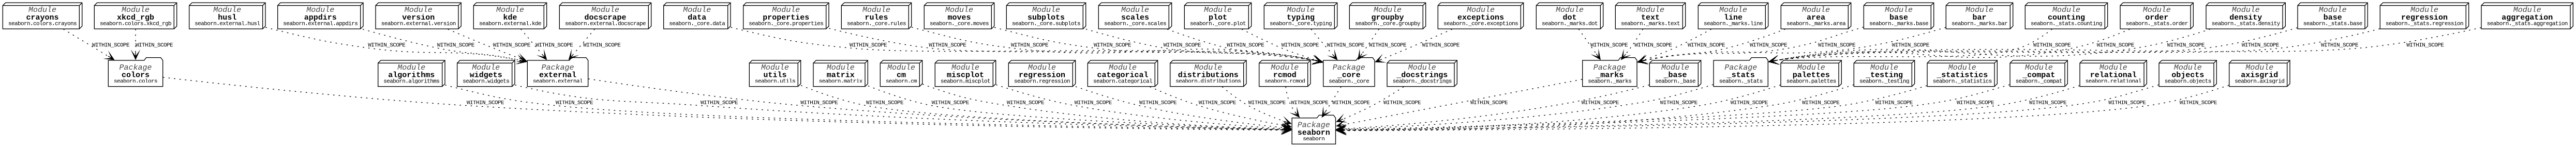
\includegraphics[angle=-90, scale=0.12]{assets/pim.png}
    \centering
    \caption{Rezultati drugog upita}
    \label{fig:upit2}
\end{figure}


\begin{figure}[h]
    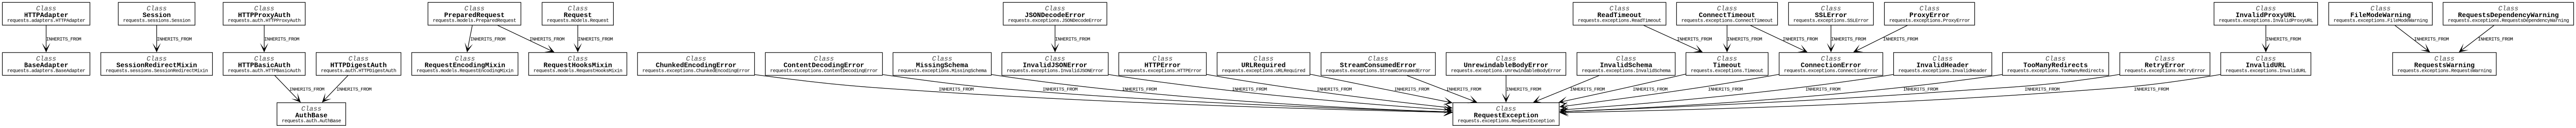
\includegraphics[angle=-90, scale=0.12]{assets/nasl.png}
    \centering
    \caption{Rezultati trećeg upita}
    \label{fig:upit3}
\end{figure}

\begin{figure}[h]
    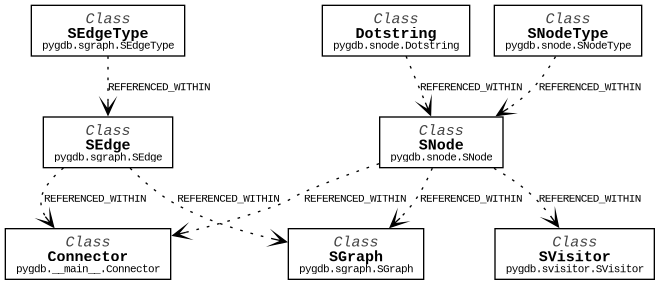
\includegraphics[scale=0.5]{assets/klref.png}
    \centering
    \caption{Rezultati četvrtog upita}
    \label{fig:upit4}
\end{figure}

\begin{table}[h]
\caption{Rezultati petog upita}
\begin{tabular}{|c|c|}
% \toprule
\hline
fullname & name \\ \hline
% \midrule
humanize.number.intcomma & intcomma \\ \hline
pymc.util.hashable & hashable \\ \hline
pymc.variational.updates.nesterov_momentum & nesterov_momentum \\ \hline
pymc.variational.updates.adamax & adamax \\ \hline
pymc.logprob.utils.convert_indices & convert_indices \\ \hline
pymc.printing._str_for_input_var & _str_for_input_var \\ \hline
pymc.variational.updates.adam & adam \\ \hline
pymc.variational.updates.adagrad & adagrad \\ \hline
pymc.variational.updates.adadelta & adadelta \\ \hline
pymc.model.fgraph.model_from_fgraph.first_non_model_var & first_non_model_var \\ \hline
pymc.distributions.multivariate.DirichletMultinomial.support_point & support_point \\ \hline
pymc.pytensorf.collect_default_updates.find_default_update & find_default_update \\ \hline
pymc.variational.updates.adagrad_window & adagrad_window \\ \hline
pymc.variational.updates.sgd & sgd \\ \hline
pymc.distributions.discrete.NegativeBinomial.logp & logp \\ \hline
pymc.model.core.Model.replace_rvs_by_values & replace_rvs_by_values \\ \hline
pymc.variational.updates.rmsprop & rmsprop \\ \hline
% \bottomrule
\end{tabular}
\label{tab:upit5}
\end{table}

\begin{figure}
    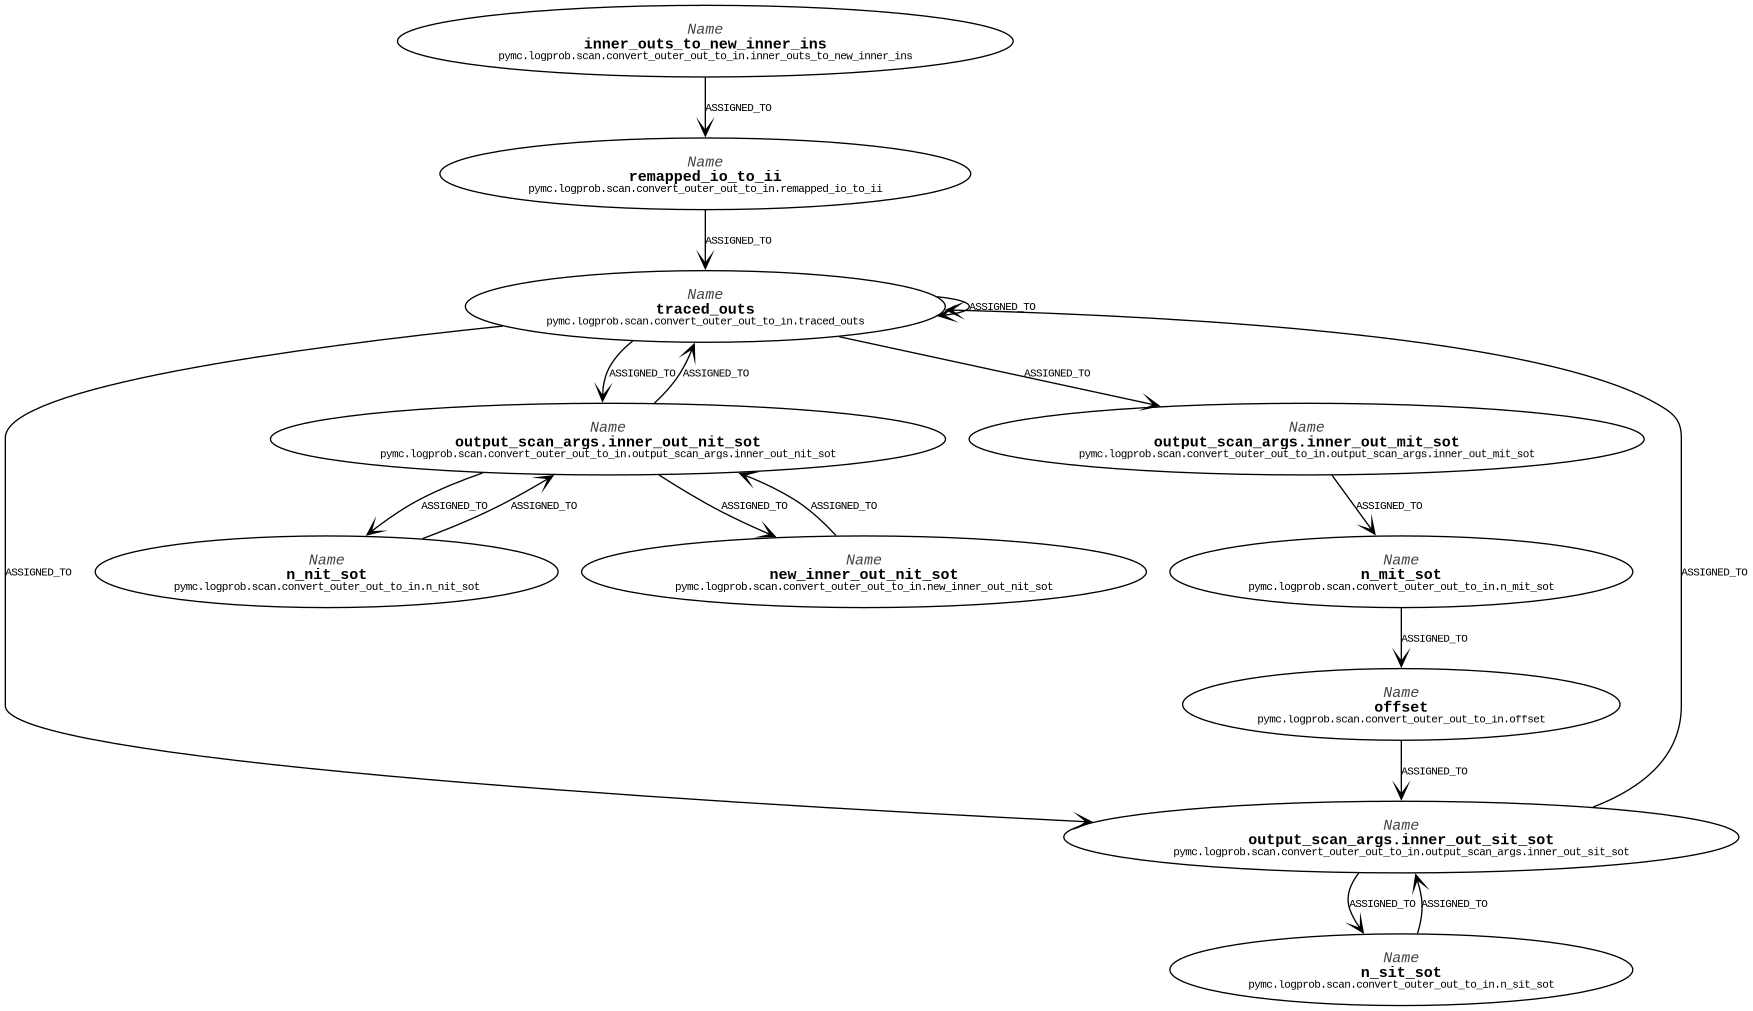
\includegraphics[scale=0.3]{assets/aschain.png}
    \centering
    \caption{Rezultati šestog upita}
    \label{fig:upit6}
\end{figure}

\begin{figure}
    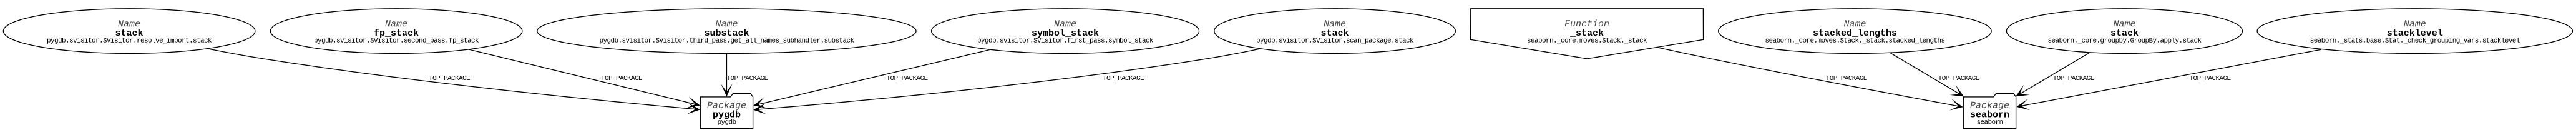
\includegraphics[scale=0.12, angle=90]{assets/stack.png}
    \centering
    \caption{Rezultati sedmog upita}
    \label{fig:upit7}
\end{figure}


\begin{figure}
    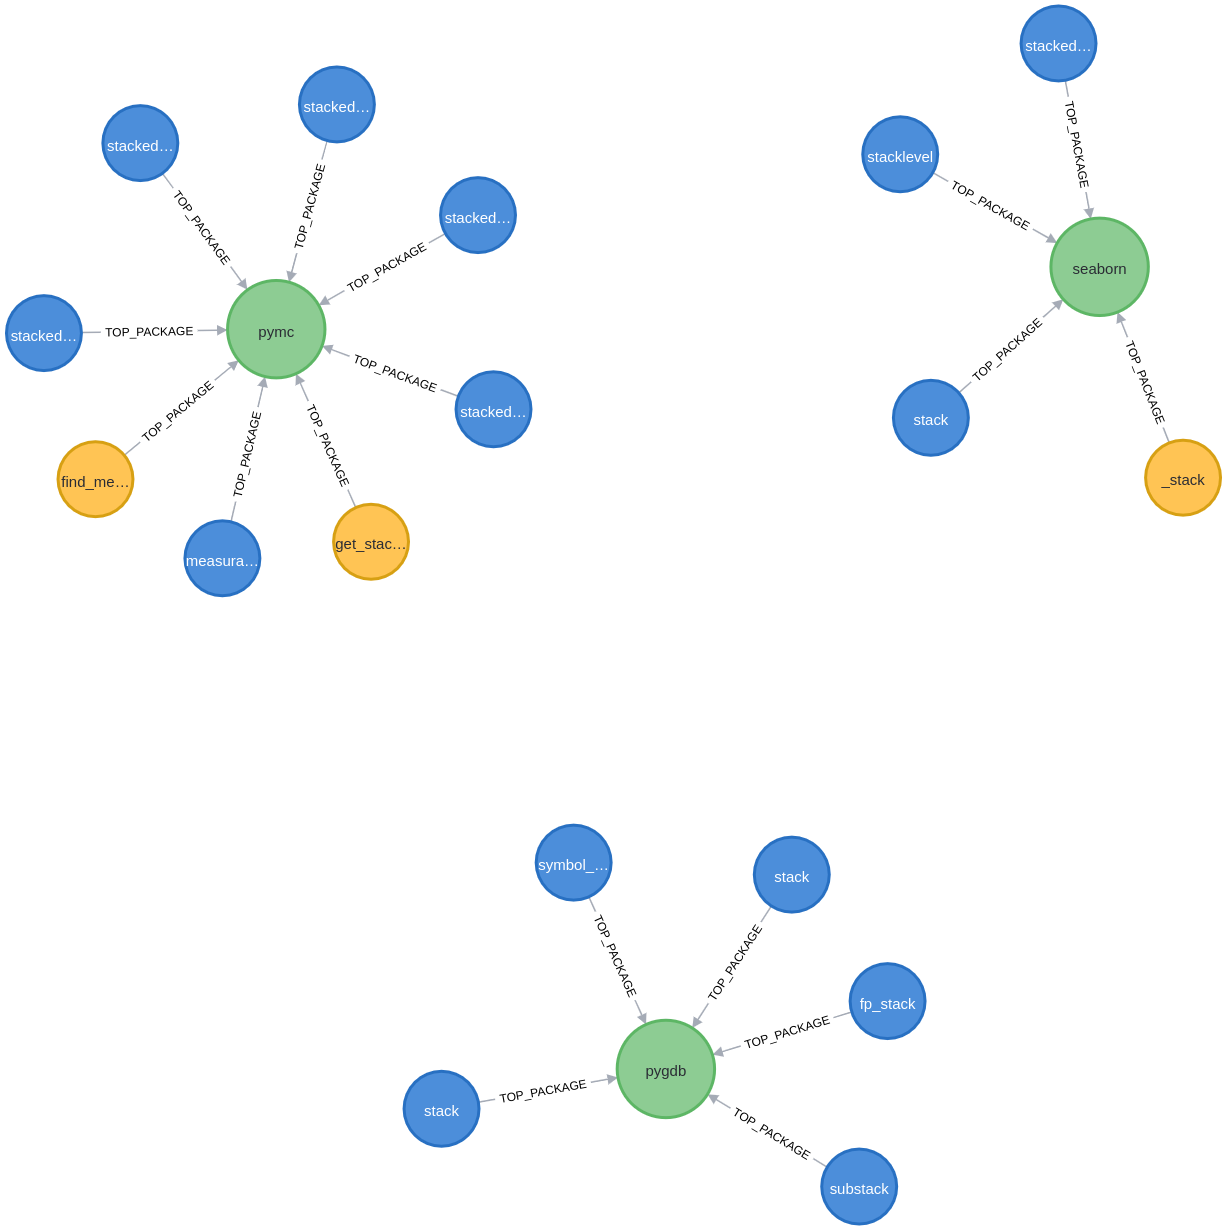
\includegraphics[scale=0.3]{assets/stack2.png}
    \centering
    \caption{Rezultati sedmog upita (puni upit, Neo4j varijanta)}
    \label{fig:upit72}
\end{figure}
